\documentclass[189]{pset}

% ================================================================== %
%                                                                    %
%                              Document                              %
%                                                                    %
% ================================================================== %

% ----------------------- Header formatting ------------------------ %

\name{Forest Kobayashi}
\class{Math of Big Data}
\season{Summer}
\prof{Gu}
\assignment{2}
\duedate{05/16/2018}
\dueday{Wednesday}
\problems{1, 2, 3}
\acknowledgements{{Murphy, Stackexchange (thread about Hessian)}, {},
  {}}
\onTime{0}

\comments{\textbf{Comments:} Feel free to work with other students,
  but make sure you write up the homework and code on your own (no
  copying homework \textit{or} code; no pair programming). Feel free
  to ask students or instructors for help debugging code or whatever
  else, though.

  The starter files can be found under the Resource tab on course
  website. The graphs for problem 3 generated by the sample solution
  could be found in the corresponding zipfile. These graphs only serve
  as references to your implementation. You should generate your own
  graphs for submission. Please print out all the graphs generated by
  your own code and submit them together with the written part, and
  make sure you upload the code to your Github repository.}

\lfoot{Due Tuesday, May 15th 2018}

\begin{document}

% --------------------------- Problem 1 ---------------------------- %

  \section{(Murphy 8.3) Gradient and Hessian of the log-likelihood for
    logistic regression.}

    \begin{enumerate}
      \item Let $\sigma(x) = \frac{1}{1 + e^{-x}}$ be the sigmoid
        function. Show that
        \[
          \sigma'(x) = \sigma(x)\bk{1 - \sigma(x)}
        \]
      \item Using the previous result and the chain rule of calculus,
        derive an expression for the gradient of the log likelihood
        for logistic regression.
      \item The Hessian can be written as $\bH=\bX^\T\bS\bX$ where
        $\bS = \diag(\mu_1(1-\mu_1), \dots, \mu_n(1-\mu_n))$. Derive
        this and show that $\bH \succeq 0$ ($A \succeq 0$ means that
        $A$ is positive semidefinite).
    \end{enumerate}

    \textit{Hint:} Use the \textbf{negative} log-likelihood of
    logistic regression for this problem.

  \hrulefill

  \section*{Solution:}
  \begin{enumerate}
    \item Note that
      \begin{align*}
        \sigma'(x)
        &= \od{}{x} \pn{1+e^{-x}}^{-1} \\
        &= -1\cdot -e^{-x} \pn{1+e^{-x}}^{-2} \\
        &= \frac{e^{-x}}{\pn{1+e^{-x}}^2} \\
        &= \frac{1}{1+e^{-x}} \cdot \frac{e^{-x}}{1 + e^{-x}} \\
        &= \sigma(x)\bk{\frac{1+e^{-x} - 1}{1+e^{-x}}} \\
        &= \sigma(x)\bk{\frac{1+e^{-x}}{1+e^{-x}} -
          \frac{1}{1+e^{-x}}} \\
        &= \sigma(x)\bk{1-\sigma(x)}
      \end{align*}
    \item We have
      \begin{align*}
        \mrm{NLL}(\vw)
        &= -\sum_{i=1}^N y_i \log\pn{h(\vx_i)} + (1-y_i)\log(1-
          h(\vx_i))
      \end{align*}
      where $h(\vx_i)=\sigma(\bm{\theta}^\T \vx_i)$. Hence
      \begin{align*}
        \nabla_{\bm{\theta}} \mrm{NLL}(\vw)
        &= -\sum_{i=1}^N \pd{}{\theta_i} \bk[Big]{ y_i
          \log\pn{h(\vx_i)} + (1-y_i)\log(1- h(\vx_i)) } \\
        &= -\sum_{i=1}^N\bk{\frac{y_i}{h(\vx_i)}\pd{h(\vx_i)}{
          \bm{\theta}} - \frac{1-y_i}{1- h(\vx_i)}h'(\vx_i)
          \pd{h(\vx_i)}{\bm{\theta}}}
      \end{align*}
      by the previous result, we have
      \[
        \pd{h(\vx_i)}{\bm{\theta}} = h(\vx_i)(1-h(\vx_i))
      \]
      hence
      \begin{align*}
        \nabla_{\bm{\theta}} \mrm{NLL}(\vw)
        &= -\sum_{i=1}^N \bk{y_i\pn{1-h(\vx_i)}\vx_i-(1-y_i)h(\vx_i)
          \vx_i} \\
        &= -\sum_{i=1}^N \bk{\vx_i \pn{y_i(1-h(\vx_i)) - (1-y_i)
          h(\vx_i)}} \\
        &= -\sum_{i=1}^N \bk{\vx_i\pn{y_i - y_ih(\vx_i) - h(\vx_i) +
          y_i h(\vx_i)}} \\
        &= -\sum_{i=1}^N \bk{\vx_i \pn{y_i - h(\vx_i)}} \\
        &= \sum_{i=1}^N \bk{\vx_i (h(\vx_i) - y_i)}
      \end{align*}
      checking with the solutions, we see that it'd be a good idea to
      define $\mu_i = \sigma(\bm{\theta}^\T \vx_i)$. Then
      \begin{align*}
        \nabla_{\bm \theta} \mrm{NLL}(\vw)
        &= \sum_{i=1}^N \vx_i \pn{\mu_i - y_i} \\
        &= \bX^\T \pn{\bm{\mu} - \vy}
      \end{align*}
    \item Let $\bJ$ denote the Jacobian matrix. Then
      \begin{align*}
        \bH(\mrm{NLL}(\vw))
        &= \bJ(\nabla_{\bm \theta} \mrm{NLL}(\vw))^\T \\
        &= \bJ(\bX^\T\pn{\bm{\mu} - \vy})^\T \\
        &= \bJ(\bX^\T \bm{\mu})^\T \\
        &= \sum_{i=1}^N \pn{\pd{\mu_i}{\bm{\theta}}} \vx_i^\T \\
        &= \sum_{i=1}^N \pn{\vx_i \pn{\mu_i(1-\mu_i)} \vx_i^\T} \\
        &= \bX^\T \diag(\mu_1(1-\mu_1), \ldots, \mu_n(1-\mu_n)) \bX \\
        &= \bX^\T \bS \bX
      \end{align*}
      Note that by the definition of $\sigma(x)$, $\forall i \in [N]$,
      $0 < \mu_i < 1$. Hence $1-\mu_i > 0$. Thus $\forall i \in [N]$,
      $\mu_i (1-\mu_i) > 0$. Now, observe that $\bS$ is the diagonal
      matrix of eigenvalues of $\bH$, which are all of the form
      $\mu_i(1-\mu_i)$. Thus, all the eigenvalues of $\bH$ are
      nonnegative, so $\bH$ is positive semidefinite. \qed
  \end{enumerate}


  \clearpage

% --------------------------- Problem 2 ---------------------------- %

  \section{(Murphy 2.11)}
    Derive the normalization constant ($Z$) for a one dimensional
    zero-mean Gaussian
    \[
      \PP(x; \sigma^2) = \frac{1}{Z}\exp\pn{-\frac{x^2}{2\sigma^2}}
    \]
    such that $\PP(x; \sigma^2)$ becomes a valid density.

  \hrulefill

  \section*{Solution:}
    For $\PP(x;\sigma^2)$ to be normalized, it must integrate to 1
    over $\RR$. Hence, we must have
    \begin{align*}
      Z
      &= \int_{-\infty}^\infty \exp\pn{-\frac{x^2}{2\sigma^2}}\dd x
    \end{align*}
    because the antiderivative is not expressable in terms of
    elementary functions, we pull out some trickery. Squaring $Z$,
    \begin{align*}
      Z^2
      &= \pn{\int_{-\infty}^\infty \exp\pn{-\frac{x^2}{2\sigma^2}}\dd
        x}^2 \\
      &= \int_{-\infty}^\infty \exp\pn{-\frac{x_0^2}{2\sigma^2}}\dd
        x_0 \int_{-\infty}^\infty \exp\pn{-\frac{x_1^2}{2\sigma^2}}\dd
        x_1 \\
      &= \int_{-\infty}^\infty \int_{-\infty}^\infty \exp\pn{-\frac{
        x_0^2 + x_1^2}{2\sigma^2}} \dd x_0 \dd x_1
    \end{align*}
    We want to convert to polar coordinates. Consider the
    transformation $x_0 \mapsto r\cos(\theta)$; $x_1 \mapsto
    r\sin(\theta)$. Then $x_0^2 + y_0^2 = r^2\pn{\cos^2\pn{\theta} +
      \sin^2\pn{\theta}} = r^2$, and by the power of Math 60 (and
    google), we recall that $\dd x \dd y \mapsto r \dd r \dd \theta$.
    Hence, our integral becomes
    \begin{align*}
      Z^2
      &= \int_0^{2\pi} \int_0^\infty r\exp\pn{-\frac{r}{2\sigma^2} \dd
        r \dd \theta} \\
      &= \int_0^{2\pi} \pn{-\sigma^2 \exp\pn{-\frac{r^2}{2\sigma^2}}
        \bigg\vert_0^\infty } \dd \theta \\
      &= \int_0^{2\pi} \sigma^2 \dd \theta \\
      &= 2\pi \sigma^2
    \end{align*}
    hence
    \[
      \boxed{Z = \sqrt{2\pi}\sigma}
    \]
    as desired. \qed

  \clearpage

% --------------------------- Problem 2 ---------------------------- %

  \section{(Regression)}
    In this problem, we will use the online news popularity dataset to
    set up a model for linear regression. In the starter code, we have
    already parsed the data for you. However, you might need internet
    connection to access the data and therefore successfully run the
    starter code.

    We split the csv file into a training and test set with the first
    two thirds of the data in the training set and the rest for
    testing. Of the testing data, we split the first half into a
    `validation set' (used to optimize hyperparameters while leaving
    your testing data pristine) and the remaining half as your test
    set. We will use this data for the remainder of the problem. The
    goal of this data is to predict the \textbf{log} number of shares
    a news article will have given the other features.

  \begin{enumerate}
    \item (\textbf{math}) Show that the maximum a posteriori problem
      for linear regression with a zero-mean Gaussian prior $\PP(\vw)
      = \prod_j \cN(w_j | 0, \tau^2)$ on the weights,
      \[
        \argmax_\vw \sum_{i=1}^N \log\cN(y_i | w_0 + \vw^\T\vx_i,
        \sigma^2) + \sum_{j=1}^D \log\cN(w_j | 0, \tau^2)
      \]
      is equivalent to the ridge regression problem
      \[
        \argmin_\vw \frac{1}{N}\sum_{i=1}^N (y_i - (w_0 +
        \vw^\T\vx_i))^2 + \lambda \norm{\vw}_2^2
      \]
      with $\lambda = \sigma^2 / \tau^2$.

    \item (\textbf{math}) Find a closed form solution $\vx^\star$ to
      the ridge regression problem:
    \[
      \text{minimize: } \norm{A\vx - \vb}_2^2 + \norm{\Gamma \vx}_2^2
    \]

  \item (\textbf{implementation}) Attempt to predict the
    $\log\text{shares}$ using ridge regression from the previous
    problem solution. Make sure you include a bias term and
    \textit{don't regularize the bias term}. Find the optimal
    regularization parameter $\lambda$ from the validation set. Plot
    both $\lambda$ versus the validation RMSE (you should have tried
    at least 150 parameter settings randomly chosen between 0.0 and
    150.0 because the dataset is small) and $\lambda$ versus
    $\norm{\bm{\theta}^\star}_2$ where $\bm{\theta}$ is your weight
    vector. What is the final RMSE on the test set with the optimal
    $\lambda^\star$?

  \item (\textbf{math}) Consider regularized linear regression where
    we pull the basis term out of the feature vectors. That is,
    instead of computing $\hat\vy = \bm{\theta}^\T\vx$ with $\vx_0 =
    1$, we compute $\hat\vy = \bm{\theta}^\T\vx + b$. This corresponds
    to solving the optimization problem
    \[
      \text{minimize: } \norm{A\vx + b\1 - \vy}_2^2 + \norm{\Gamma
        \vx}_2^2
    \]
    Solve for the optimal $\vx^\star$ explicitly. Use this close form
    to compute the bias term for the previous problem (with the same
    regularization strategy). Make sure it is the same.
  \item (\textbf{implementation}) We can also compute the solution to
    the least squares problem using gradient descent. Consider the
    same bias-relocated objective
    \[
      \text{minimize: } f = \norm{A\vx + b\1 - \vy}_2^2 + \norm{\Gamma
      \vx}_2^2
    \]
    Compute the gradients and run gradient descent. Plot the $\ell_2$
    norm between the optimal $(\vx^\star, b^\star)$ vector you
    computed in closed form and the iterates generated by gradient
    descent.

    \textit{Hint:} your plot should move down and to the left and
    approach zero as the number of iterations increases. If it
    doesn't, try decreasing the learning rate.
  \end{enumerate}

  \hrulefill

  \clearpage

  \section*{Solution:}
    \begin{enumerate}
      \item Substituting in our expression for the standard normal
        probability distribution, we have
        \begin{align*}
          \mrm{MAP}(\vx)
          &= \argmax_{\vw} \sum_{i=1}^N \bk{
            \log\pn{\frac{1}{\sqrt{2\pi}\sigma} \exp\pn{
            -\frac{\pn{y_i - (w_0 + \vw^\T \vx_i)}^2}{2\sigma^2}}}} +
            \sum_{j=1}^D \bk{\log\pn{\frac{1}{\sqrt{2\pi}\sigma}
            \exp\pn{-\frac{ w_j^2}{2\tau^2}}}} \\
          &= \argmax_{\vw} \sum_{i=1}^N
            \bk{\log{\frac{1}{\sqrt{2\pi}\sigma}} - \frac{\pn{y_i -
            \pn{w_0 + \vw^\T \vx_i}}^2}{2\sigma^2}} + \sum_{j=1}^D
            \bk{\log\pn{\frac{1}{\sqrt{2\pi}\tau}} -
            \frac{w_j^2}{2\tau^2}}
            \shortintertext{The constants don't matter (independent of
            $\vw$), so we ignore them.}
          &= \argmax_{\vw} \sum_{i=1}^N \bk{-\frac{\pn{y_i - (w_0 +
            \vw^\T \vx_i)}^2}{2\sigma^2}} + \sum_{j=1}^D
            \bk{-\frac{w_j^2}{2\tau^2}}
            \shortintertext{multiplying out by $2\sigma^2$, we obtain}
          2\sigma^2\mrm{MAP}(\vx)
          &= \sum_{i=1}^N \bk{-(y_i - (w_0 + \vw^\T \vx_i)^2)} +
            \frac{\sigma^2}{\tau^2} \sum_{j=1}^D \bk{-w_j^2} \\
          &= -\pn{\sum_{i=1}^N \bk{\pn{y_i - (w_0 + \vw^\T \vx_i)}^2}
            + \lambda \sum_{j=1}^D \bk{w_j^2}}
            \shortintertext{by definition of $\ell_2$ norm, this
            becomes}
            &= -\pn{\sum_{i=1}^N \bk{\pn{y_i - (w_0 + \vw^\T \vx_i)}^2
             } + \lambda \norm{\vw}_2^2}
        \end{align*}
        $\mrm{MAP}(\vx)$ is maximized when the part inside the parens
        is minimized, hence we seek to solve the following estimation
        problem:
        \begin{align*}
          \Theta(\vw)
          &= \argmin_{\vw} \sum_{i=1}^N \pn{y_i - (w_0 + \vw^\T
            \vx_i)}^2 + \lambda \norm{\vw}_2^2
        \end{align*}
        Supposedly, I'm missing a factor of $1/N$. But, without
        redefining $\lambda$, I don't see how I could obtain one.
      \item First, we prove a small lemma.
        \begin{lemma}
          Let $\vx \in \RR^n$, and $A \in \mc{L}(\RR^n)$. Then
          $\nabla_{\vx} \pn{\vx^\T A \vx} = \vx^\T \pn{A + A^\T}$.
        \end{lemma}
        \begin{proof}
          By the product rule, we have
          \begin{align*}
            \nabla_{\vx} \pn{\vx^\T A \vx}
            &= \pn{\nabla_{\vx}\pn{\vx^\T}} A \vx + \vx^\T A
              \pn{\nabla_{\vx} \pn{\vx}}
              \shortintertext{because these are all $1\times 1$
              matrices, they are symmetric, hence}
            &= \pn{\nabla_{\vx}\pn{\vx^\T}} A \vx + \pn{\vx^\T A
              \pn{\nabla_{\vx} \pn{\vx}}}^\T \\
            &= \pn{\nabla_{\vx}\pn{\vx^\T}} A\vx +
              \pn{\nabla_{\vx}\pn{\vx}}^\T A^\T \vx \\
            &= \pn{\nabla_{\vx}\pn{\vx^\T}} A\vx +
              \pn{\nabla_{\vx}\pn{\vx^\T}} A^\T\vx \\
            &= \nabla_{\vx} \pn{\vx^\T} \pn{A + A^\T}\vx \\
            &= 1\cdot \pn{A + A^\T}\vx
          \end{align*}
          as desired.
        \end{proof}
        Now, we proceed to the main problem. By the definition of
        $\ell_2$ norm, we have
        \begin{align*}
          f(\vx)
          &= \norm{A\vx - \vb}_2^2 + \norm{\Gamma \vx }_2^2\\
          &= \vx^\T A^\T A \vx - \vx^\T A^\T \vb - \vb^\T A \vx +
            \vx^\T \Gamma^\T \Gamma \vx + \vb^\T \vb
        \end{align*}
        we want to minimize $f(\vx)$. Hence, we set the gradient to 0.
        Note that the $\vb^\T \vb$ goes away.
        \begin{align*}
          \nabla_{\vx} f(\vx)
          &= \nabla_{\vx} \pn{\vx^\T A^\T A \vx - \vx^\T A^\T \vb -
            \vb^\T A \vx + \vx^\T \Gamma^\T \Gamma \vx} \\
          &= \nabla_{\vx} \pn{\vx^\T \pn{A^\T A + \Gamma^\T \Gamma}\vx
            - \pn{\vx^\T A^\T \vb + \pn{\vx^\T A^\T \vb}^\T}}
            \shortintertext{since these will all be $1\times 1$
            matrices, they'll all be symmetric, hence $\vx^\T A^\T \vb
            = (\vx^\T A^\T \vb)^\T$. Thus,}
          &= \nabla_{\vx} \pn{\vx^\T \pn{A^\T A + \Gamma^\T \Gamma}\vx
            - 2\vx^\T A^\T\vb}
            \shortintertext{by the lemma,}
          &= \pn{A^\T A + \Gamma^\T \Gamma + AA^\T +
            \Gamma\Gamma^\T}\vx - 2A^\T \vb \\
          &= 2(A^\T A + \Gamma^\T \Gamma)\vx - 2A^\T \vb \\
          &= 0
        \end{align*}
        hence,
        \begin{align*}
          2(A^\T A + \Gamma^\T \Gamma)\vx
          &= 2A^\T \vb \\
          (A^\T A + \Gamma^\T \Gamma)\vx
          &= A^\T \vb
        \end{align*}
        suppose $(A^\T A + \Gamma^\T \Gamma)$ is invertible. Then
        \[
          \boxed{\vx = \pn{A^\T A + \Gamma^\T \Gamma}^{-1} A^\T \vb}
        \]
        having looked at the coding portion and become confused, I
        checked the answer key, and saw that we were supposed to
        state that in the special case where $\Gamma = \sqrt{\lambda}
        I$, we obtain an expression of the form
        \[
          \boxed{\vx = \pn{A^\T A + \lambda I}^{-1} A^\T \vb}
        \]
      \item We find $\lambda^\star = 8.5361$, with RMSE on the test
        set being $.8628$. See plots on next page.
        \begin{figure}[H]
          \centering
          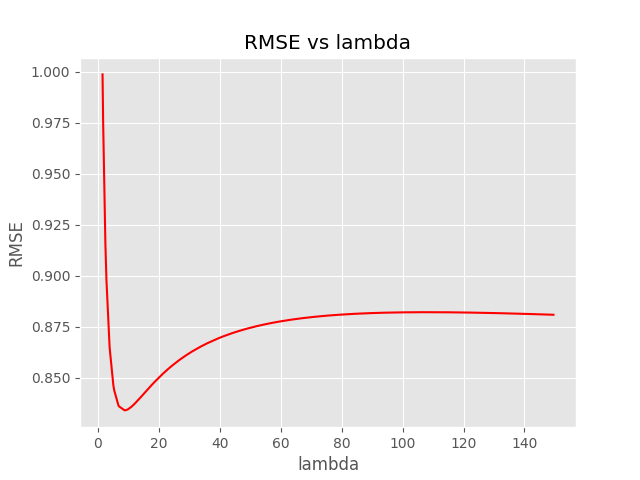
\includegraphics[width=13cm]{RMSE_vs_lambda.png}
          \caption{RMSE vs. $\lambda$}
          \label{fig:rmsvl}
        \end{figure}
        \begin{figure}[H]
          \centering
          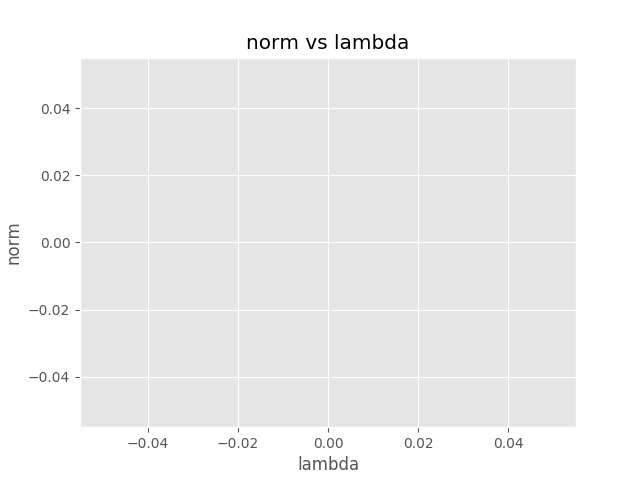
\includegraphics[width=13cm]{norm_vs_lambda.png}
          \caption{$\norm{\bm{\theta}^\star}_2^2$ vs. $\lambda$}
          \label{fig:fdsa}
        \end{figure}
      \item I'm still a little unclear about why we can't recycle our
        answer from (b). Anyways, we want to minimize
        \begin{align*}
          f(\vx)
          &= \pn{A\vx + b\1 - \vy}^\T \pn{A\vx + b\1 - \vy} + \vx^\T
            \Gamma^\T \Gamma \vx \\
          &= \vx^\T A^\T A \vx + \vx^\T A^\T b\1 - \vx^\T A^\T \vy +
            b\1^\T A\vx + b^2 \1^\T \1 - b\1^\T \vy - \vy^\T A\vx -
            \vy^\T b\1 + \vy^\T \vy + \vx^\T \Gamma^\T \Gamma \vx
        \end{align*}
        hence
        \begin{align*}
          \nabla_\vx f
          &= 2(A^\T A + \Gamma^\T \Gamma) \vx + A^\T\pn{2b\1-2\vy}\\
          &= 0
        \end{align*}
        and
        \begin{align*}
          \nabla_b f
          &= 2\vx^\T A^\T \1 + 2bn - 2\1^\T \vy \\
          &= 0
        \end{align*}
        thus, rearranging terms, transposing the $\vx$ term and
        dividing by $2n$, we have
        \begin{align*}
          b^\star
          &= \frac{\1^\T\pn{\vy - A\vx}}{n}
        \end{align*}
        plugging back into the $\nabla_\vx$ equation, we have
        \begin{align*}
          0
          &= \pn{A^\T A + \Gamma^\T \Gamma}\vx + A^\T \pn{\frac{
            \1\1^\T\pn{\vy - A\vx}}{n} - \vy} \\
          &= \pn{A^\T A + \Gamma^\T \Gamma}\vx + \frac{1}{n} A^\T \1
            \1^\T \vy - \frac{1}{n}A^\T \1\1^\T A\vx -
            A^\T \vy \\
          &= \pn{A^\T A + \Gamma^\T \Gamma - \frac{1}{n}A^\T \1\1^\T
            A}\vx + \frac{1}{n} A^\T \1 \1^\T \vy - A^\T \vy
        \end{align*}
        hence
        \begin{align*}
          \pn{A^\T A + \Gamma^\T \Gamma - \frac{1}{n}A^\T \1\1^\T
          A}\vx
          &= A^\T \vy - \frac{1}{n} A^\T \1 \1^\T \vy \\
          &= \pn{A^\T - \frac{1}{n}A^\T \1\1^\T}\vy
        \end{align*}
        and so
        \begin{align*}
          \vx^\star
          &= \pn{A^\T A + \Gamma^\T \Gamma - \frac{1}{n}A^\T \1\1^\T
            A}^{-1} \pn{A^\T - \frac{1}{n}A^\T \1\1^\T}\vy \\
          &= \boxed{\pn{A^\T \bk{I - \frac{1}{n}\1\1^\T}A +
            \Gamma^\T\Gamma}^{-1} A^\T \pn{I - \frac{1}{n}\1\1^\T}\vy}
        \end{align*}
        this yields a difference in bias of just $3.3939 \cdot
        10^{-11}$, with the difference in weights being similar.
        Success!
        % By part (b), we see that
        % \[
        %   \boxed{\vx = \pn{A^\T A + \Gamma^\T \Gamma}^{-1}A^\T \pn{b\1
        %       - \vy}}
        % \]
      \item
    \end{enumerate}

\end{document}
